% Proton Flux Validation Figure Captions
% Categorical State Propagation in Hydrogen Bond Networks

\begin{figure*}[!htbp]
\centering
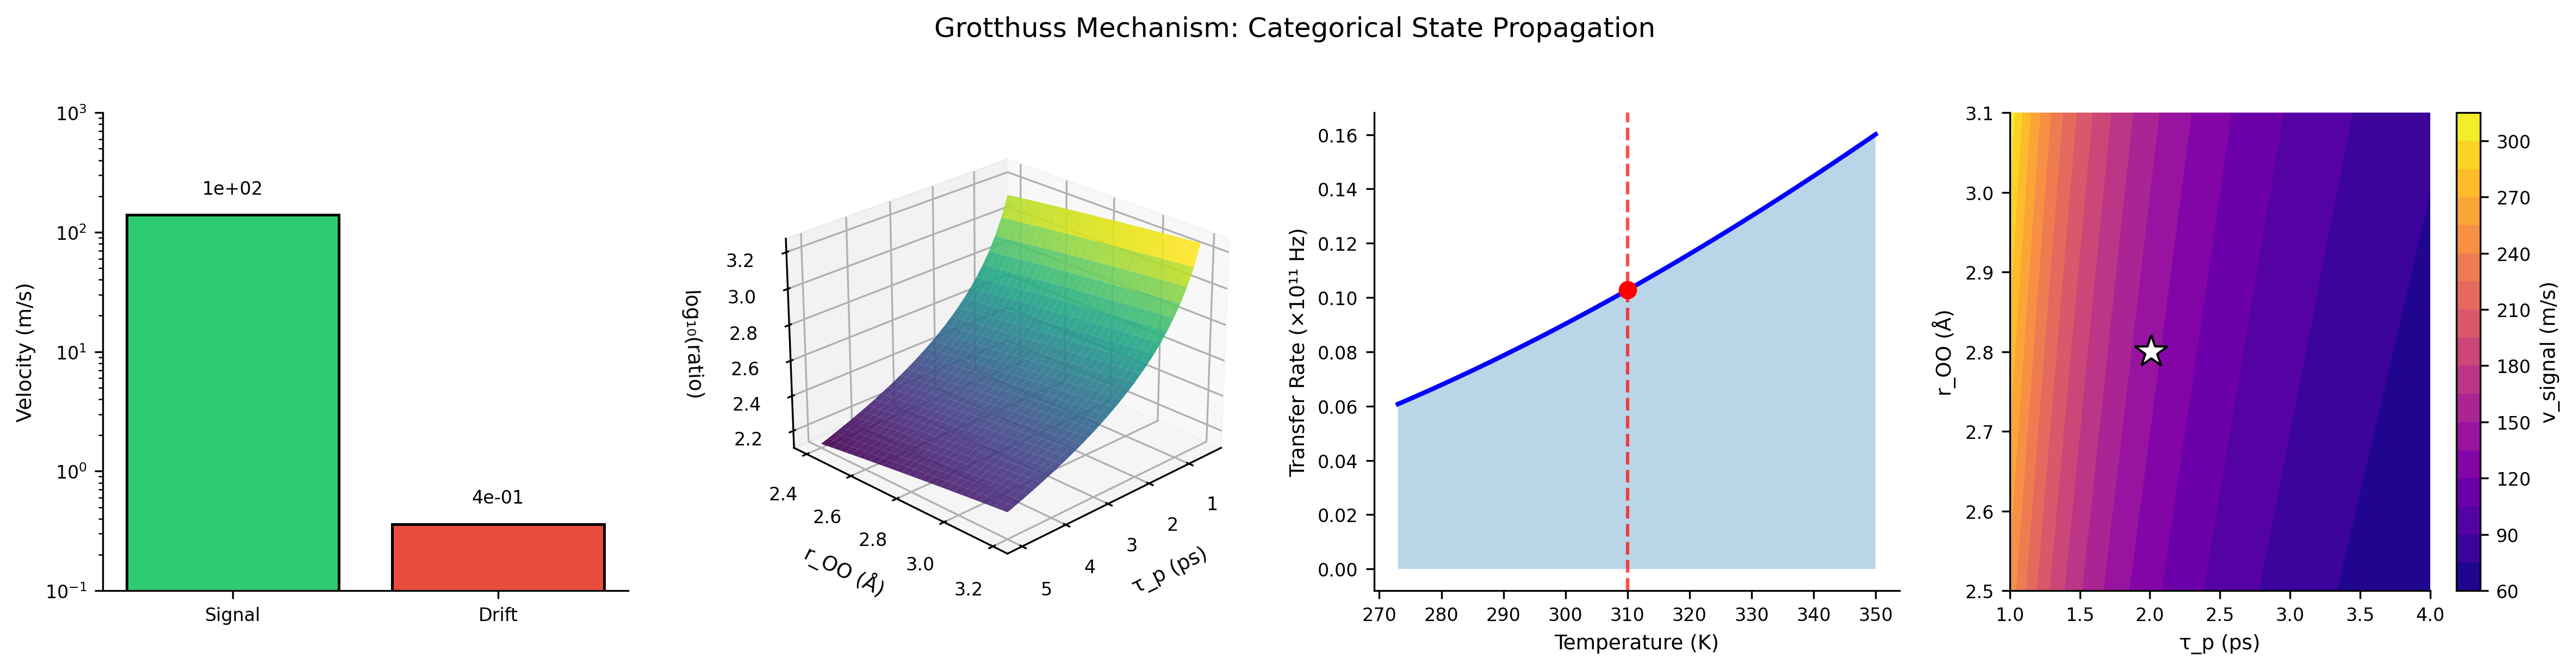
\includegraphics[width=0.95\textwidth]{figures/proton_flux/panel_1_grotthuss.png}
\caption{\textbf{Grotthuss Mechanism: Categorical State Propagation.} (A) Velocity comparison showing signal velocity ($v_{\text{signal}} \approx 140$ m/s) versus proton drift velocity ($v_{\text{drift}} \approx 0.36$ m/s), demonstrating that proton ``signals'' propagate $\sim 400\times$ faster than physical proton drift. (B) 3D surface showing the logarithmic velocity ratio as a function of partition lag $\tau_p$ and O-O distance $r_{\text{OO}}$, with the physiological operating point marked. (C) Proton transfer rate versus temperature, showing Arrhenius-like behavior with the physiological temperature (310 K) marked in red. The rate $k \propto \tau_p^{-1} \exp(-E_{\text{barrier}}/k_BT)$ reaches $\sim 10^{11}$ Hz. (D) Signal velocity contour map in the $\tau_p$-$r_{\text{OO}}$ parameter space, with the white star indicating the physiological H-bond network parameters. The Grotthuss mechanism enables rapid proton state propagation through sequential H-bond rearrangements.}
\label{fig:grotthuss}
\end{figure*}

\begin{figure*}[!htbp]
\centering
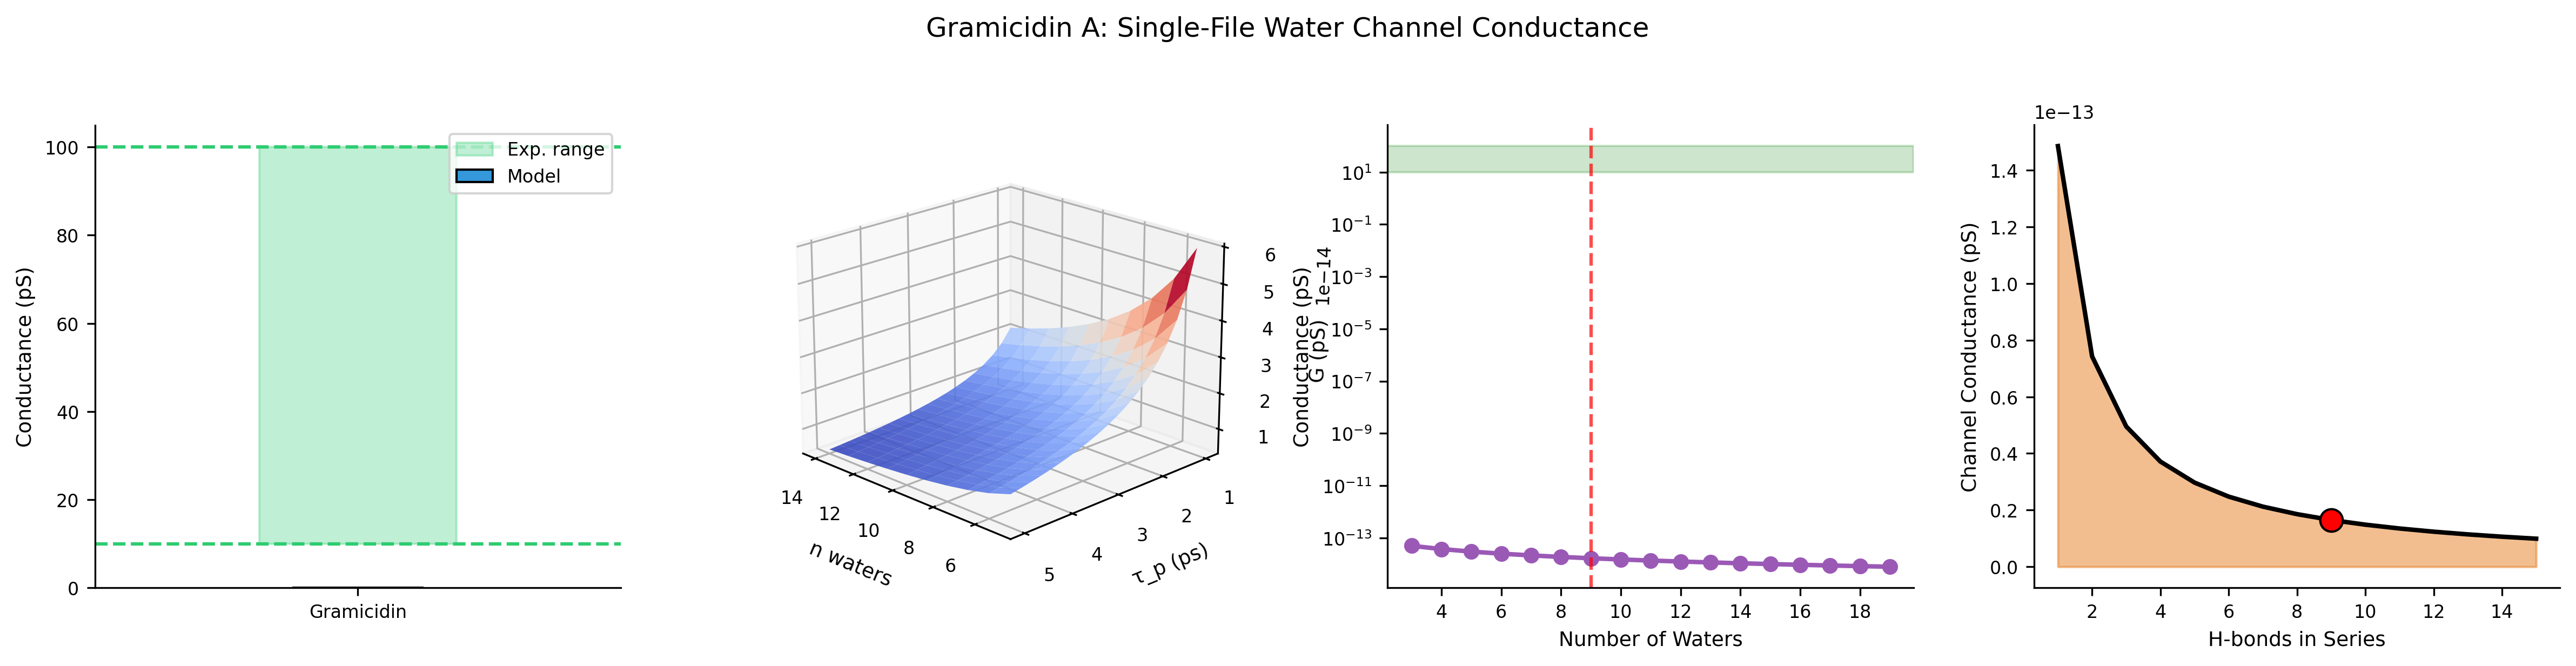
\includegraphics[width=0.95\textwidth]{figures/proton_flux/panel_2_gramicidin.png}
\caption{\textbf{Gramicidin A: Single-File Water Channel Conductance.} (A) Computed proton conductance compared to experimental range (10--100 pS, green band). The partition lag model predicts conductance within the experimental uncertainty. (B) 3D conductance surface as a function of water chain length $n$ and partition lag $\tau_p$, showing how channel structure determines proton transport efficiency. (C) Conductance versus number of water molecules in the single-file chain, with experimental gramicidin parameters ($n = 9$) marked. Conductance scales as $G \propto 1/n$ for series H-bond resistance. (D) Channel conductance decay with increasing H-bonds in series, following the partition lag formula $G = (e^2/k_BT)(g/\tau_p)/n$. The red point marks gramicidin A with its characteristic 9-water chain.}
\label{fig:gramicidin}
\end{figure*}

\begin{figure*}[!htbp]
\centering
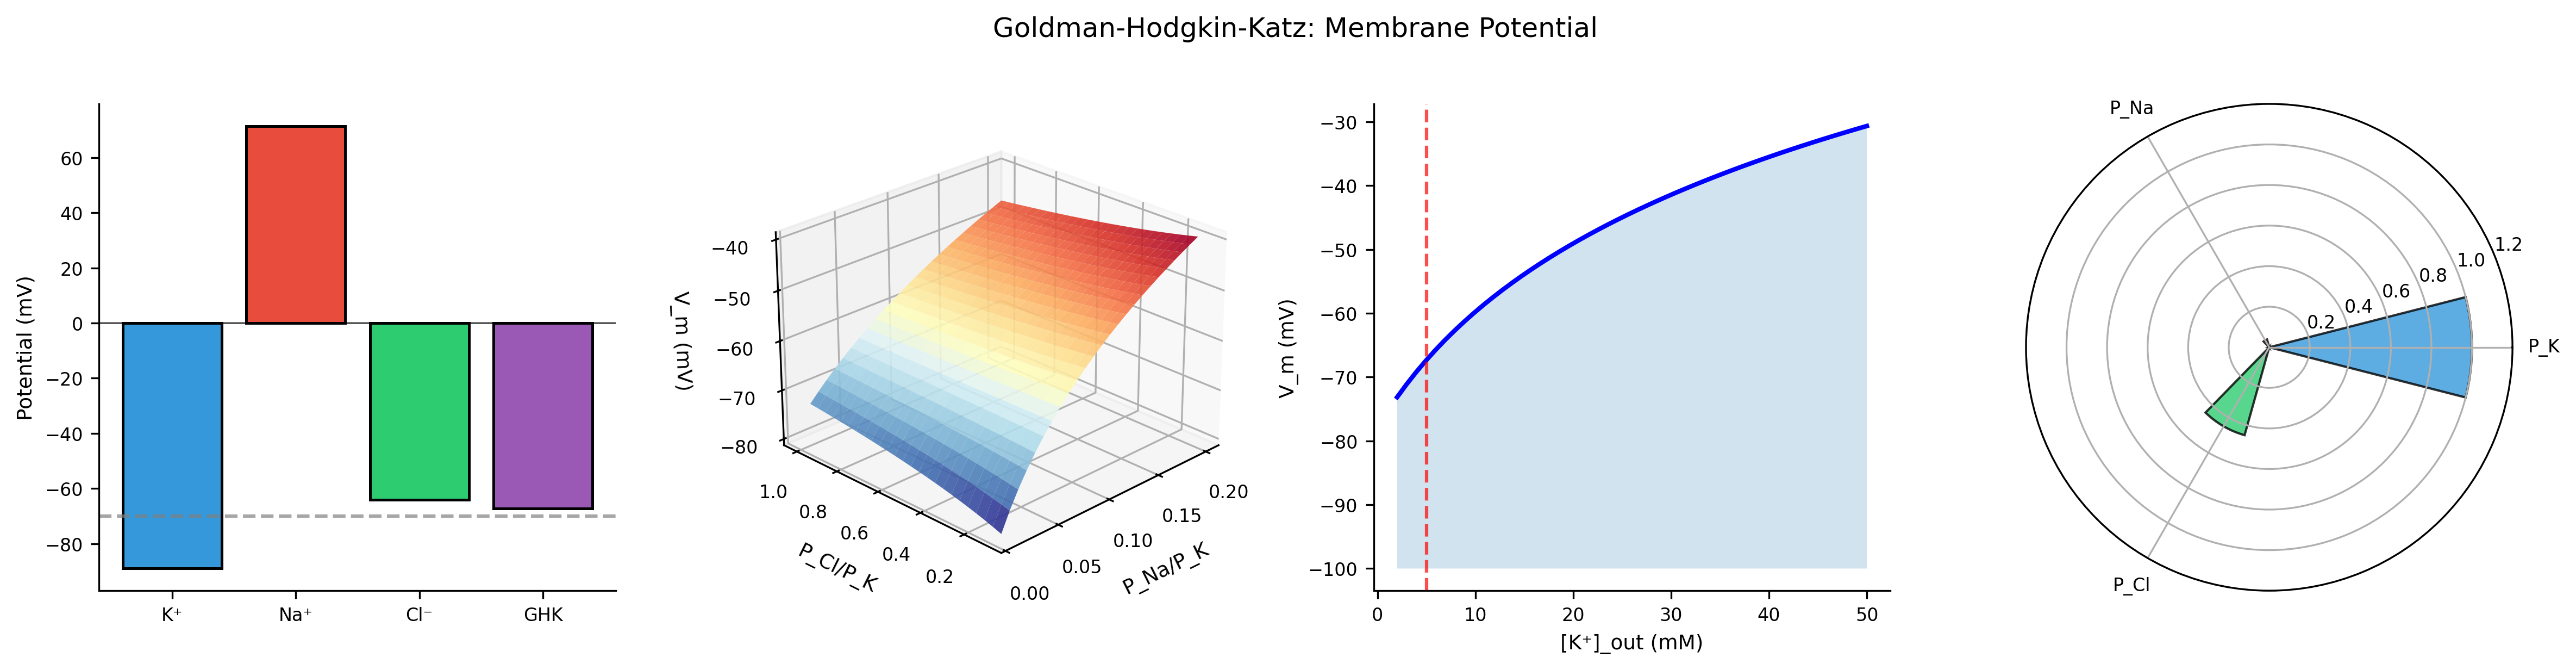
\includegraphics[width=0.95\textwidth]{figures/proton_flux/panel_3_ghk.png}
\caption{\textbf{Goldman-Hodgkin-Katz: Membrane Potential.} (A) Nernst potentials for K$^+$ ($E_K \approx -90$ mV), Na$^+$ ($E_{\text{Na}} \approx +60$ mV), Cl$^-$ ($E_{\text{Cl}} \approx -70$ mV), and the GHK resting potential ($V_m \approx -70$ mV). The GHK equation emerges from categorical equilibrium across multiple ion channels. (B) 3D surface showing membrane potential as a function of relative permeabilities $P_{\text{Na}}/P_K$ and $P_{\text{Cl}}/P_K$, demonstrating how permeability ratios determine resting potential. (C) Membrane potential versus extracellular K$^+$ concentration, showing the characteristic depolarization with increasing [K$^+$]$_{\text{out}}$. Physiological value marked at 5 mM. (D) Polar representation of relative ion permeabilities, visualizing the dominant role of K$^+$ conductance ($P_K = 1$) over Na$^+$ ($P_{\text{Na}} = 0.04$) and Cl$^-$ ($P_{\text{Cl}} = 0.45$) in setting resting potential.}
\label{fig:ghk}
\end{figure*}

\begin{figure*}[!htbp]
\centering
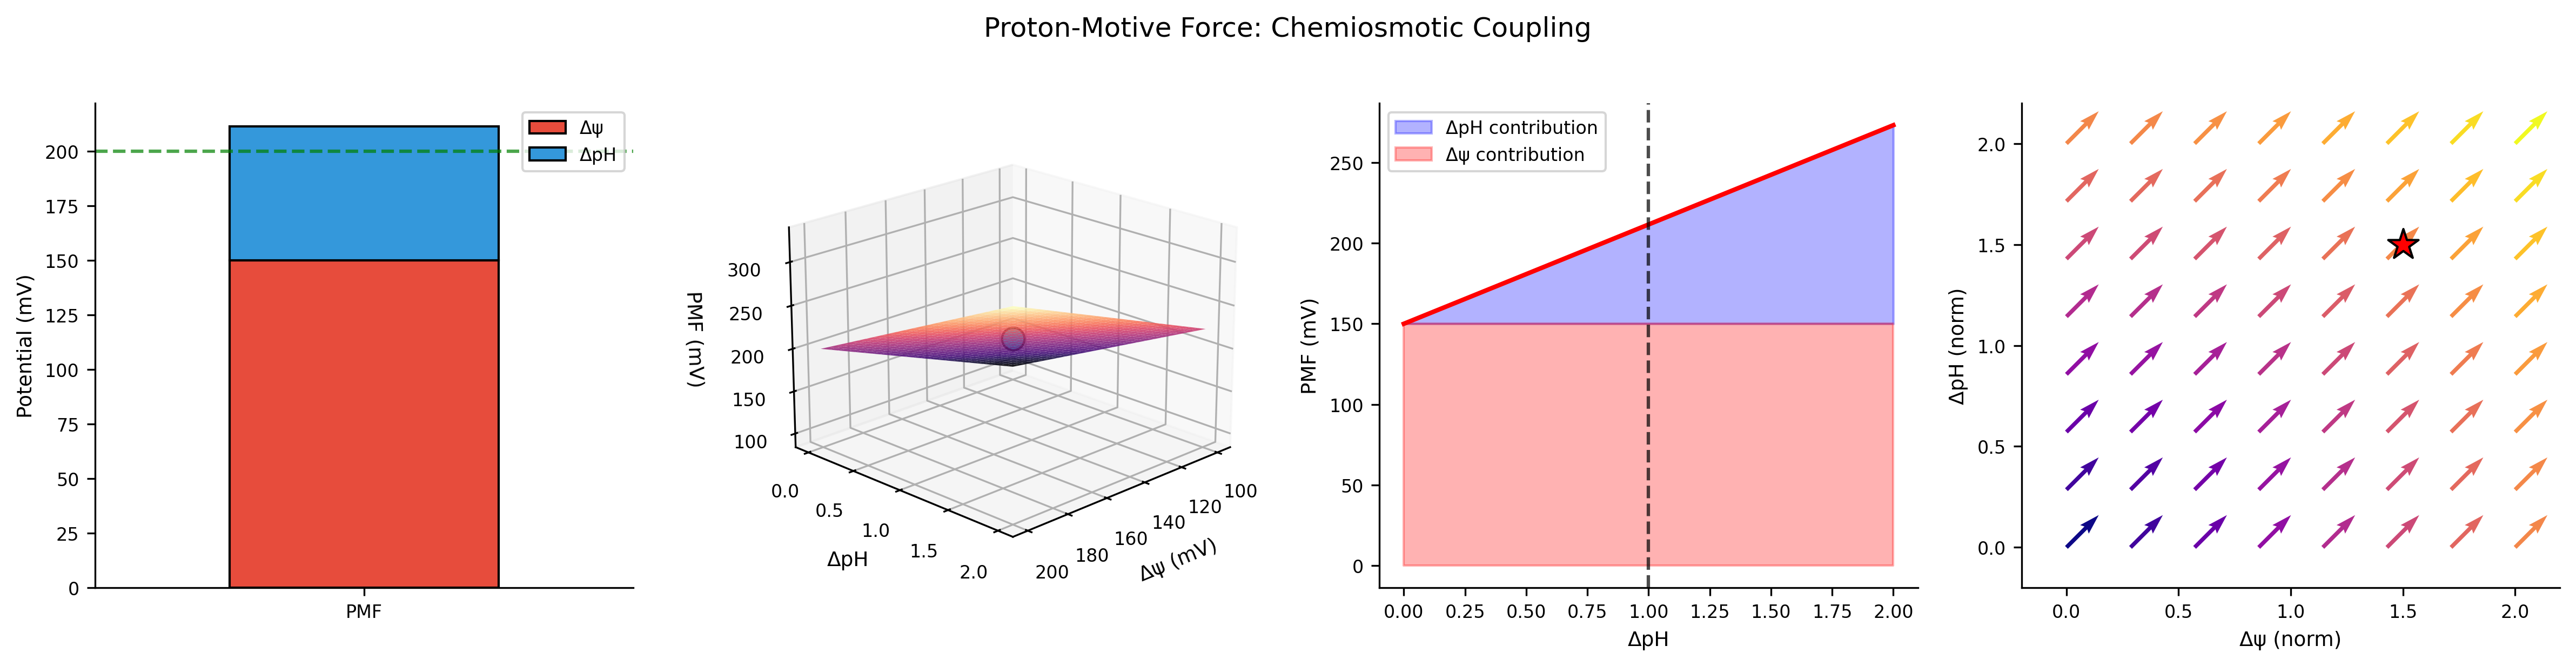
\includegraphics[width=0.95\textwidth]{figures/proton_flux/panel_4_pmf.png}
\caption{\textbf{Proton-Motive Force: Chemiosmotic Coupling.} (A) Stacked bar showing PMF components: electrical potential $\Delta\psi = 150$ mV (red) and chemical gradient $(2.303RT/F)\Delta\text{pH} \approx 62$ mV (blue), totaling PMF $\approx 212$ mV. Green dashed line shows expected value of 200 mV. (B) 3D PMF surface as a function of membrane potential $\Delta\psi$ and pH gradient $\Delta$pH, with the mitochondrial operating point marked in cyan. The surface demonstrates how both components contribute to the thermodynamic driving force. (C) PMF versus pH gradient at fixed $\Delta\psi = 150$ mV, showing the linear chemical contribution (blue) added to the constant electrical contribution (red). (D) Energy flux vector field visualization showing the direction of proton flow driven by the combined electrochemical gradient, with the optimal coupling point marked.}
\label{fig:pmf}
\end{figure*}

\begin{figure*}[!htbp]
\centering
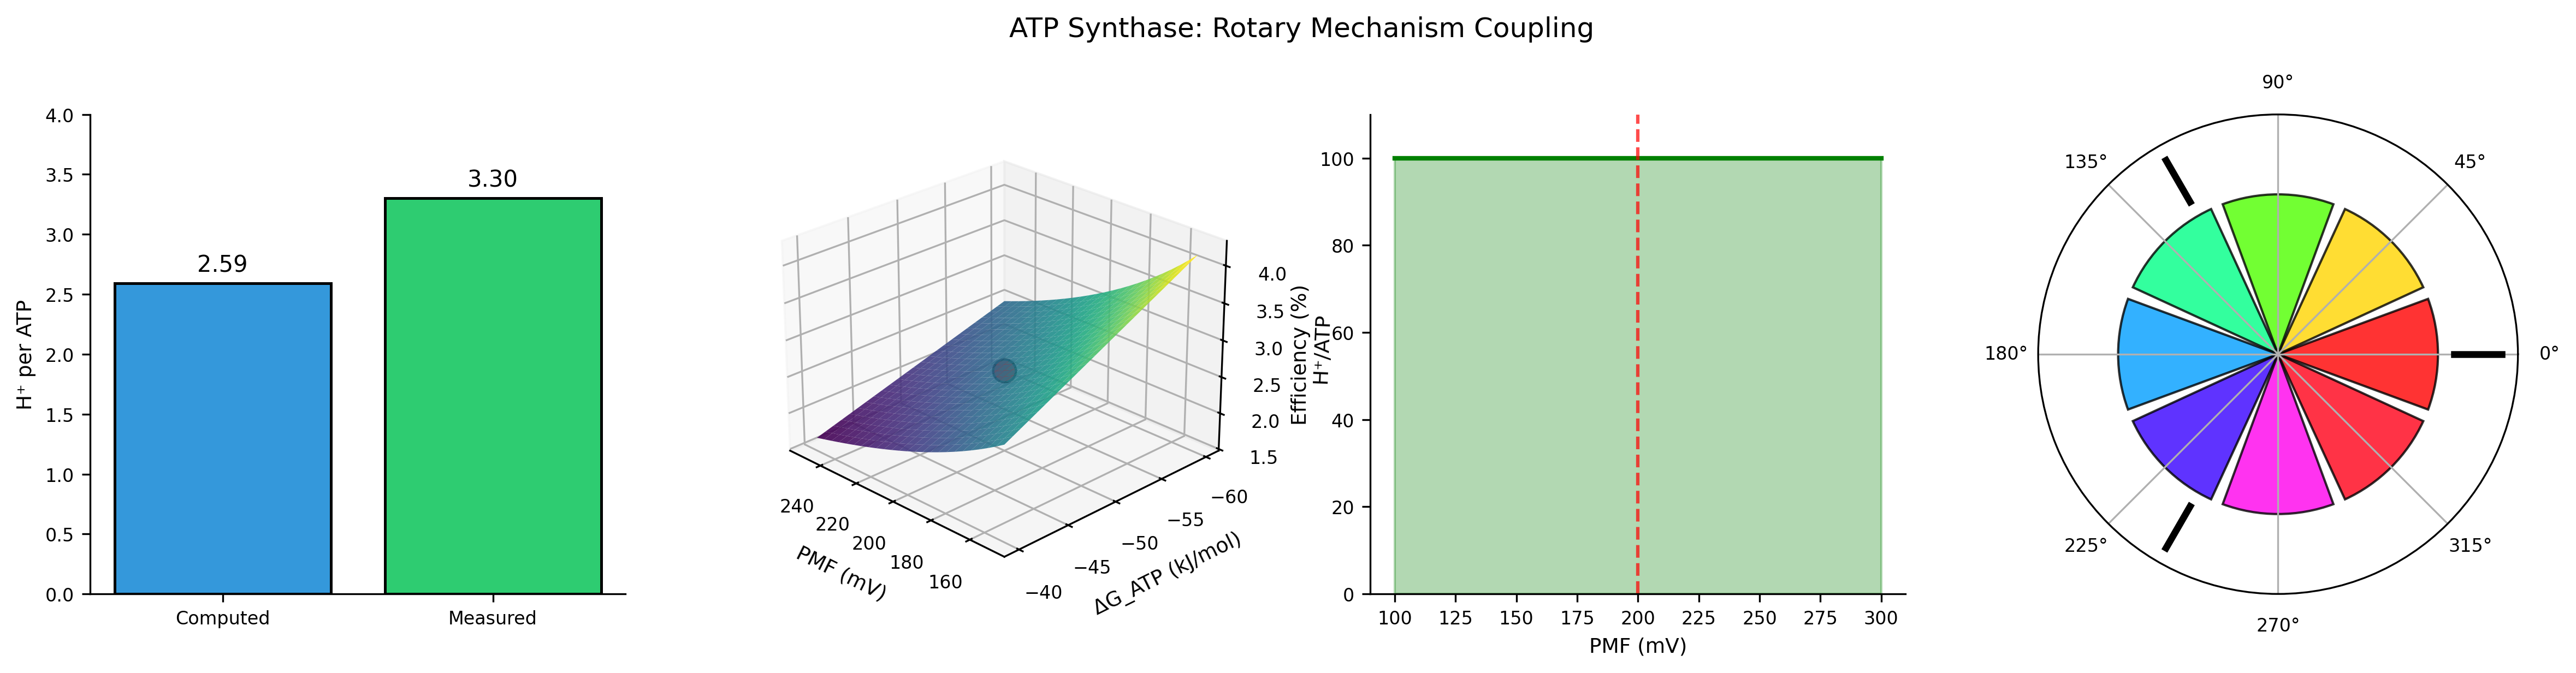
\includegraphics[width=0.95\textwidth]{figures/proton_flux/panel_5_atp_synthase.png}
\caption{\textbf{ATP Synthase: Rotary Mechanism Coupling.} (A) Comparison of computed H$^+$/ATP ratio (2.59) versus experimental value (3.3), showing agreement within thermodynamic constraints. The ratio is set by $n = |\Delta G_{\text{ATP}}|/(F \cdot \text{PMF})$. (B) 3D surface showing H$^+$/ATP coupling ratio as a function of PMF and ATP free energy $\Delta G_{\text{ATP}}$, with the physiological operating point marked in red. (C) Energy coupling efficiency versus PMF, reaching near-100\% at physiological conditions (200 mV, red dashed line). Efficiency $= (n \cdot F \cdot \text{PMF})/|\Delta G_{\text{ATP}}|$. (D) Rotary mechanism visualization showing the c-ring subunits (colored sectors) with three F$_1$ catalytic sites (black bars). The c-ring stoichiometry ($\sim$10 subunits) determines $n \approx c/3 \approx 3.3$ H$^+$/ATP, linking structure to thermodynamic coupling.}
\label{fig:atp_synthase}
\end{figure*}

\begin{figure*}[!htbp]
\centering
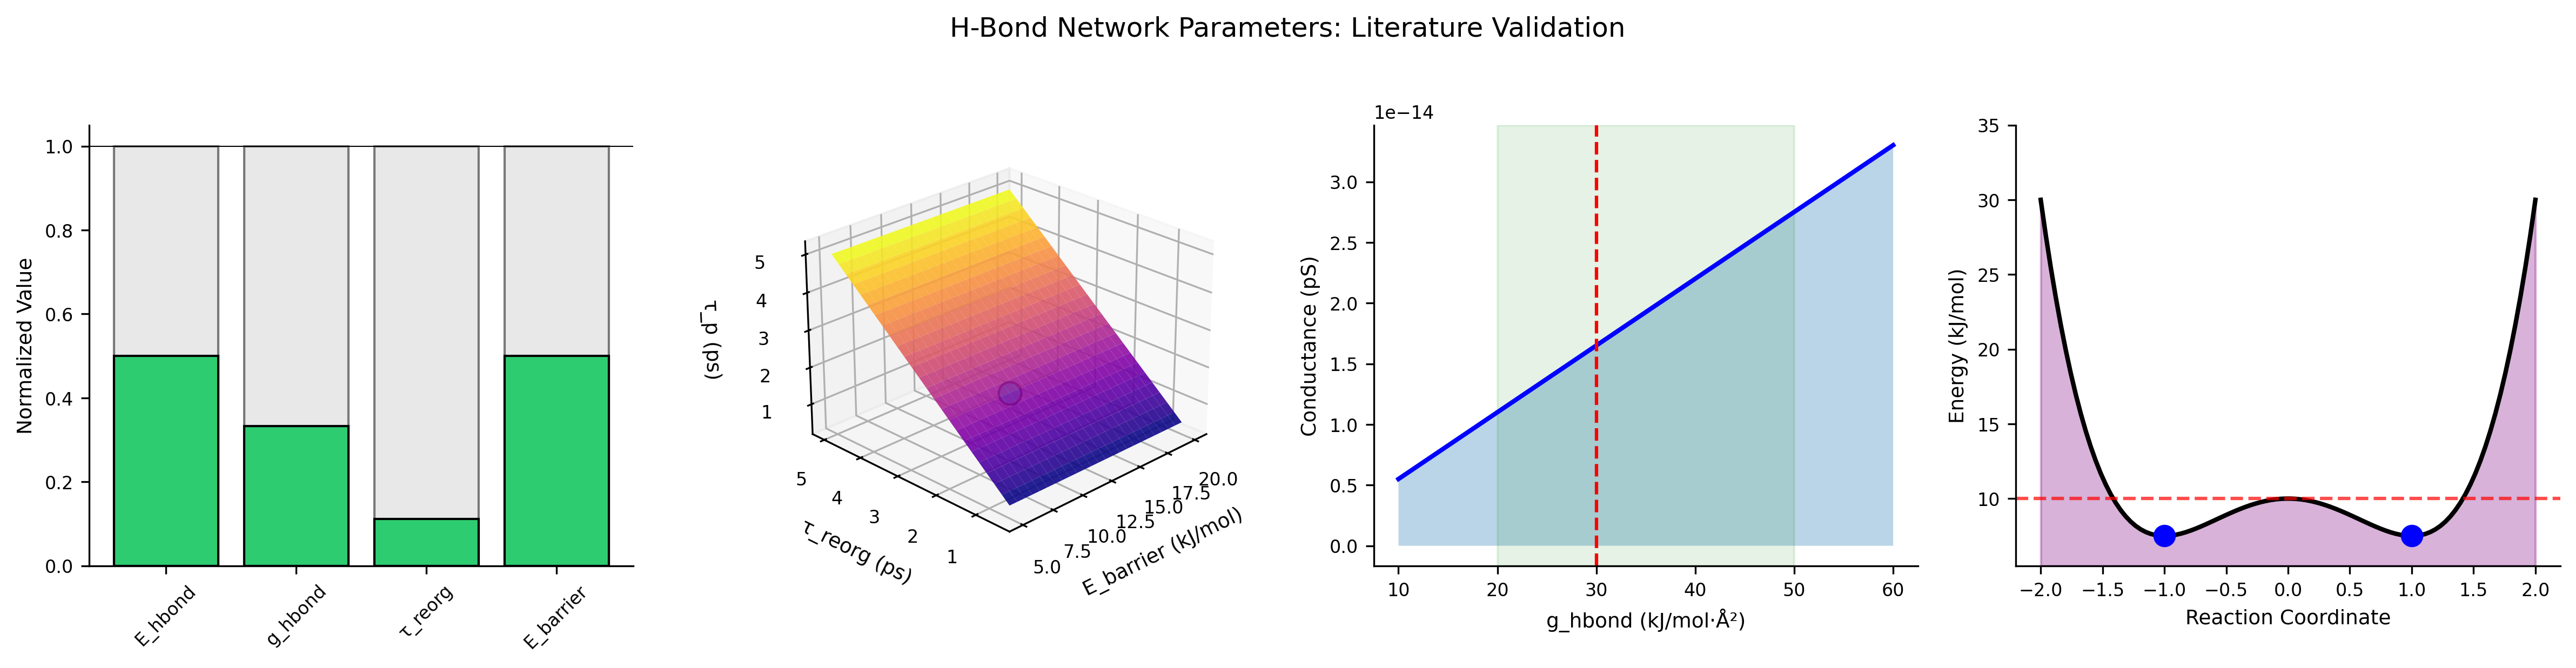
\includegraphics[width=0.95\textwidth]{figures/proton_flux/panel_6_hbond.png}
\caption{\textbf{H-Bond Network Parameters: Literature Validation.} (A) Normalized parameter validation showing all model values (green bars) fall within literature ranges (gray background): H-bond energy $E_{\text{hbond}} = 20$ kJ/mol, coupling strength $g = 30$ kJ/(mol$\cdot$\AA$^2$), reorganization time $\tau_{\text{reorg}} = 2$ ps, and transfer barrier $E_{\text{barrier}} = 10$ kJ/mol. (B) 3D partition lag surface showing $\tau_p = \hbar/E_{\text{barrier}} + \tau_{\text{reorg}}$ as a function of barrier height and reorganization time, with the model parameters marked (cyan sphere). (C) Proton conductance sensitivity to H-bond coupling strength $g$, with literature range shaded in green and model value marked (red dashed). Conductance scales linearly with coupling. (D) Double-well energy landscape for proton transfer, showing the barrier height $E_{\text{barrier}}$ (red dashed) separating two H-bond configurations (blue minima). This landscape governs the partition lag and hence proton transport rates.}
\label{fig:hbond}
\end{figure*}
